%%%%%%%%%%%%%%%%%%%%%%%%%%%%%%%%%%%%%%%%%%%%%%%%%%%%%%%%%%%
\section{Concluding remarks}
%%%%%%%%%%%%%%%%%%%%%%%%%%%%%%%%%%%%%%%%%%%%%%%%%%%%%%%%%%%
%
\begin{frame}[negative]
	\sectionpage
\end{frame}
%
%
\begin{frame}
	{Are there other ways to solve previous problems?\footnote{most also apply for previous examples, but are beyond the scope of this document (for now)}}
	
	many other (much more complex) ways,
	%
	\begin{itemize}
		%
		\item sensitivity analysis \\
		%{\small (example \hyperlink{sa}{here})}
		%
		\item post-stratification? \\
		%{\small (example \hyperlink{sa}{here})}
		%
		\item matching?
		%
		\item inverse-probability weighting?
		%
		\item g-formula?
		%
		\item g-estimations?
		%
	\end{itemize}
	%
\end{frame}
%
%
\begin{lhframe}[rhgraphic={
\includegraphics[scale=0.5]{think1.jpg}}]
	{Concluding remarks}
	
	\begin{itemize}
		%
		\item research is filled with challenges \\
		{\small (you: duh!!) }
		%
		\item statistical models are not theory \\
		{\small (you: so obvious again!!) }
		%
		\item \textcolor{blue}{don't trust} your statistical model when no DAG is involved \\
		{\small (me: how about that?!) }
		%
		\item for \textcolor{blue}{explanation}, without a DAG the (sample) size does not matter \\
		{\small (me: sorry?!) }
		%
		\item even a good experimental design \textcolor{blue}{can lead you to wrong conclusions} if no DAG is involved \\
		{\small (me: did you expect this one?!)}
		%
	\end{itemize} 
	%
\end{lhframe}
%
%
\begin{lhframe}[rhgraphic={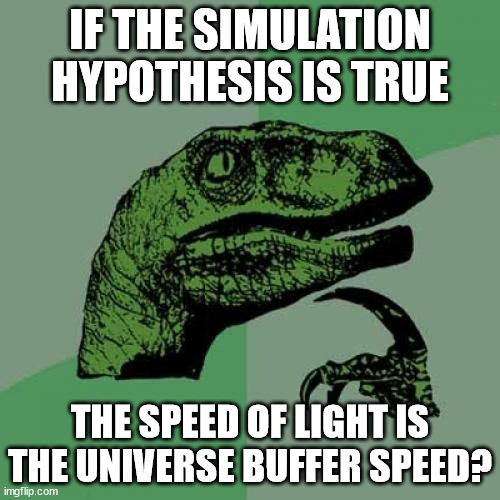
\includegraphics[scale=0.35]{think2.jpg}}]
	{Concluding remarks}
	
	Additionally, simulation can serve as,
	%
	\begin{itemize}
		%
		\item a reflection of a hypothesis, and its research complexities\\
		{\small (me: with DAGs baby!!)}
		%
		\item a place where you can reflect the status of a population \\
		{\small (test ``what happens if") }
		%
		\item a data where you can test your statistical model \\
		{\small (parameter recovery, power) }
		%
		\item a tool for planning (all kinds of) experiments.
		%
	\end{itemize} 
	%
\end{lhframe}
%
%